\documentclass{article}
\usepackage{graphicx} % Required for inserting images
\usepackage[backend=biber]{biblatex}
\addbibresource{bibliography.bib}

\title{Machine Learning For Data Science I, \\[0.1cm] Homework 03}

\author{Maj Gaberšček, 27212075}
\date{March 2023}

\begin{document}

\maketitle

\section{Problem}

The problem of this homework was to implement \textbf{Ridge (L2)} and \textbf{Lasso (L1)} regressions. Then we had to apply the Ridge regression on the superconductivity dataset and find the best regularization weight. 

\section{Ridge regression}

Ridge regression in implemented in code as a class \texttt{RidgeReg}. When initializing the object, we pass it the argument \texttt{weight}.

First method of this class is \texttt{fit}, that fits the model to the data and returns nothing. Firstly we append another column of value 1 to learning dataset $X$. This is because we want an output $y(x_1, ..., x_r) = x_1 \beta_{1} + ... + x_r \beta_{r} + \beta_{r+1}$ (the column of ones will serve to determine $\beta_{r+1}$). Then we use the closed-form solution to calculate vector $\beta$.
$$\beta=(X^T X+ \lambda I)^{-1} X^T y.$$

Second method of this class is \texttt{predict}, that returns predictions of the model on a new dataset, if the model has been fitted before that. We can find predictions, by simply adding a column of ones to the new dataset and then making a dot product with previously calculated $\beta$ vector. 

\section{Lasso regression}

Lasso regression is implemented in code as a class \texttt{LassoReg}.

Again, the first method of the model is \texttt{fit}. For similar reasons as before, we append another column of ones to the input dataset \texttt{X}. Then we minimize the function 
$$L(\beta)= \sum_{i=1}^{n}{(\beta^T x_i - y_i)^2} + \lambda \sum_{i=1}^{k}{\beta_i^2}$$
with the function \texttt{minimize} from \texttt{scipy} package. We are using the Powell method. 

The second method, \texttt{predict}, works similarly as in Ridge regression.

\section{Application}

\subsection{Superconductivity dataset}

Firstly, we loaded the dataset and split it into features, test attribute, test target, train attribute and train target values with function \texttt{load}.

Then we trained the model for different $\lambda$ values, from 0 to 3. We saved root mean squared error for each model. Then we chose the weight, that produced the lowest root mean squared error and trained the model with this weight (optimal weight was 0). We then estimated the true root mean squared error by testing the model on last 100 data (that was not used for training). RMSE estimate on testing set was was 40.7 (RMSE on training set was expectedly lower, 10.3). Plot of RMSE for different weights (tested on training data) can be seen in Figure \ref{fig:f}.

\begin{figure}[!h]
    \centering
    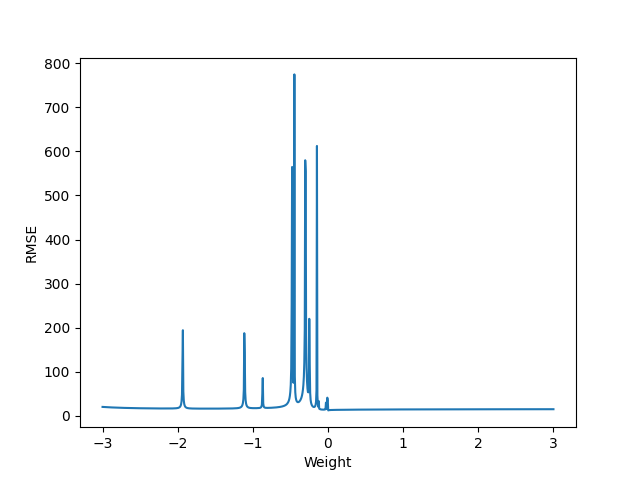
\includegraphics[width=0.7\textwidth]{homework-03/plots/ridge.png}
    \caption{RMSE for different $\lambda$ (weight) of L2 regression}
    \label{fig:f}
\end{figure}

\subsection{Tests}

At the end, we run some tests for Lasso and Ridge regression for:
\begin{itemize}
    \item small input dataset (one feature)
    \item larger training (three features)
    \item error handling, if predicting on untrained model
\end{itemize}

\printbibliography

\end{document}